\documentclass{article}
\usepackage[italian]{babel}

\usepackage{epigraph}
\usepackage{fontspec}
\usepackage{graphicx}
\usepackage[hidelinks]{hyperref}
\usepackage{verbatim}
\usepackage{graphicx}

\graphicspath{ {./images/} }

\title{
	\textbf{
		Birdazzone \\
	}
	\textbf{\large
		Relazione del progetto per l'insegnamento di \break
		Ingegneria del software
	}
}

\author{
	Paolo Ceroni (\#978232), \\
	Gabriele Crestanello (\#970352), \\
	Mattia Girolimetto (\#977478), \\
	Federica Grisendi (\#974711), \\
	Stefano Volpe (\#969766)
}

\date{
	Alma Mater Studiorum - Universit\`a di Bologna \\
	\today
}

\begin{document}

\maketitle

\epigraph{
	Engineering --- where the semi-skilled laborers execute the vision of those
	who think and dream. Hello, Oompa-Loompas of science.
}{\textit{Sheldon Cooper}}

\thispagestyle{empty}
\pagebreak

\tableofcontents

\pagebreak

\section{Descrizione del prodotto}

\subsection{\emph{Scope e backlog} di prodotto}

Le storie effettivamente svolte sono organizzate in epiche di origine.
All'interno di ciascuna epica, le storie sono organizzate in ordine decrescente
di priorità.

\subsubsection{Preparazione tecnica}

\begin{itemize}
	\item \#0 Partita a Scrumble
	\item \#1 Ambiente di sviluppo CAS
	\item \#2 Configurazione dipendente dalle tecnologie
	\item \#3 Ambiente di \emph{test}
\end{itemize}

\subsubsection{Indovinare la ``ghigliottina''}

\begin{itemize}
	\item \#4 ``Come giocatore da casa, voglio essere a conoscenza della soluzione
	      della partita per capire se ho indovintato o meno''
	\item \#5 ``Come giocatore da casa, voglio visualizzare al classifica di chi ha
	      indovinato per vedere la posizione mia e dei miei amici''
	\item \#6 ``Come giocatore da casa, voglio che solo i giocatori che hanno davvero
	      indovinato vengano mostrati in classifica''
	\item \#7 ``Come appassionato curioso, voglio visualizzare dove si trovano i
	      giocatori che hanno indovinato per studiare la loro demografia''
	\item \#8 ``Come appassionato curioso, voglio filtrare i risultati temporalmente
	      per studiare uno specifico intervallo di tempo''
	\item \#9 ``Come appassionato curioso, voglio vedere lo storico dei risultati
	      complessivi delle partite per studiare la loro evoluzione''
\end{itemize}

\subsubsection{Indovinare la ``reazione a catena''}

Questa epica, in seguito abbandonata dal cliente, ha dato origine a un gioco
segnaposto: Birdazzone, in cui si indovina in quale città una certa foto su
Twitter è stata scattata. Le storie di questa epica sono le stesse della
Ghigliottina.

\subsubsection{Fantacitorio}

\begin{itemize}
	\item \#10 ``Come giocatore del Fantacitorio, voglio vedere quanti punti ciascun
	      politico ha realizzato per capire come stia andando la partita''
	\item \#11 ``Come giocatore del Fantacitorio, voglio vedere le squadre degli altri
	      giocatori per poterle confrontare con la mia''
	\item \#12 ``Come giocatore del Fantacitorio, voglio vedere statistiche aggiuntive
	      sui politici per strategizzare meglio''
\end{itemize}

\subsubsection{Scacchi contro la folla}

\begin{itemize}
	\item \#13 ``Come giocatore di scacchi, voglio poter sfidare una folla di
	      utenti Tweeter per giocare una partita le cui mosse avversarie siano
	      decise a maggioranza''
	\item \#14 ``Come giocatore di scacchi, voglio poter condividere le mie mosse
	      su Twitter per rendere le mie partite pubbliche''
\end{itemize}

\subsection{Diagramma dei casi d'uso}

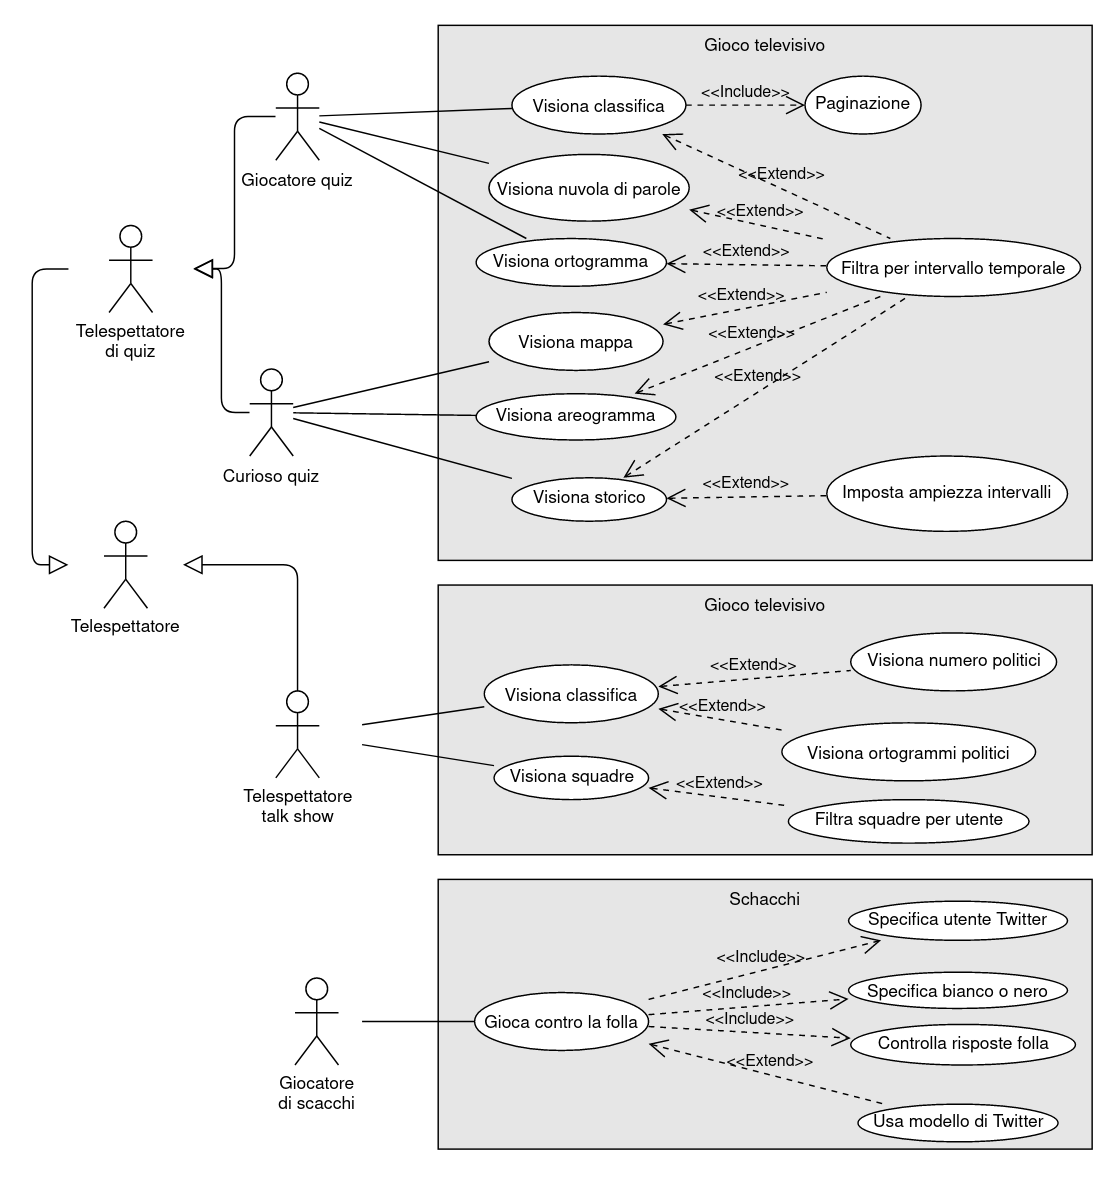
\includegraphics[width=\textwidth]{use-cases}

\subsection{Diagramma delle classi o degli oggetti}

Golang supporta la programmazione orientata agli oggetti, ma non le classi.
TypeScript supporta le classi, ma come ragionevole convenzione di progetto è
stata fatta la scelta di evitare la programmazione a oggetti durante lo
sviluppo front-end, che descrive solo una interfaccia grafica, e non la logica
di business. Ecco un diagramma pseudo-UML che descrive invece il progetto
back-end:

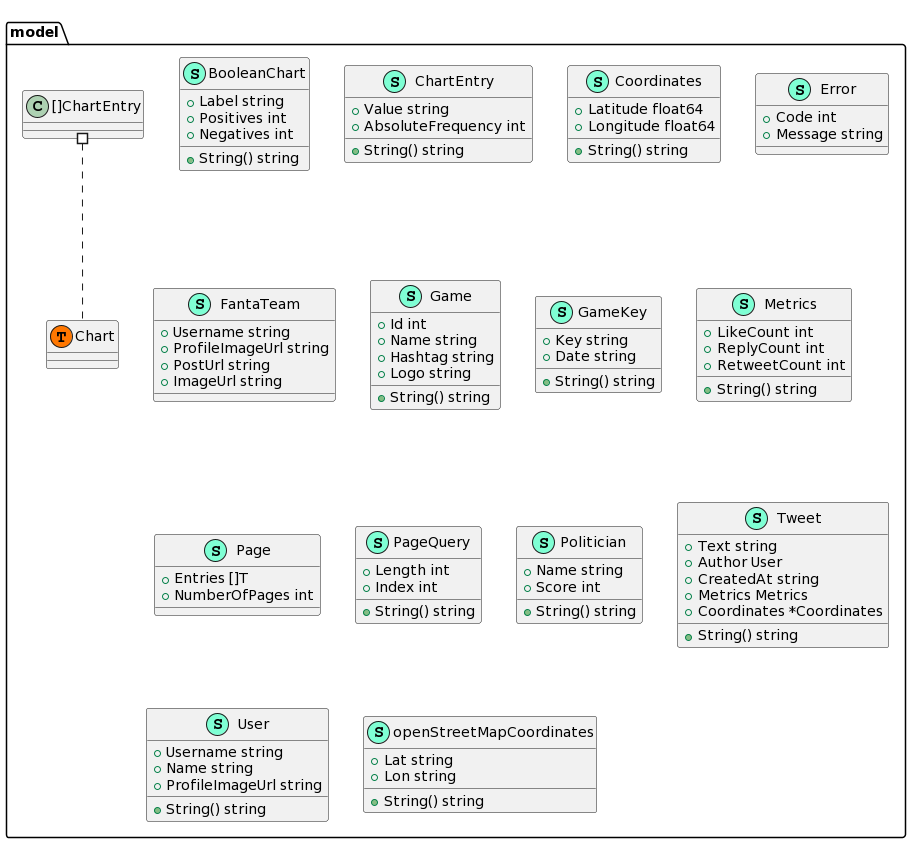
\includegraphics[width=\textwidth]{backend-model}
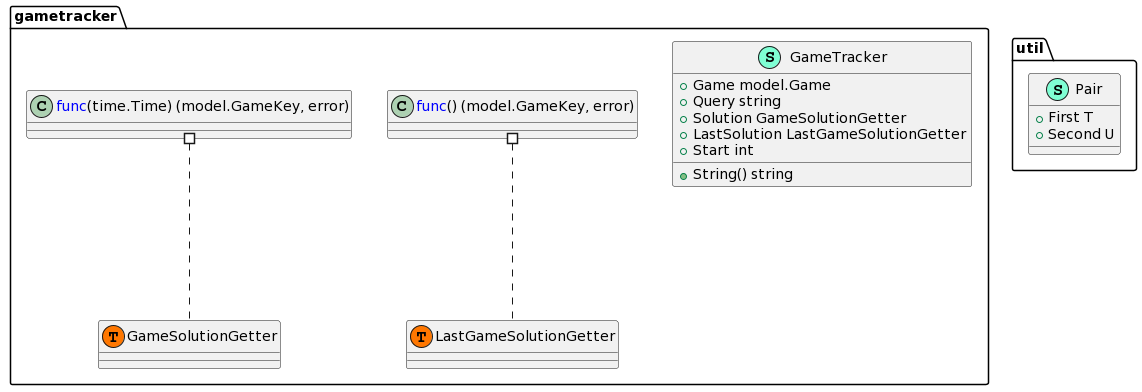
\includegraphics[width=\textwidth]{backend-gametracker-util}
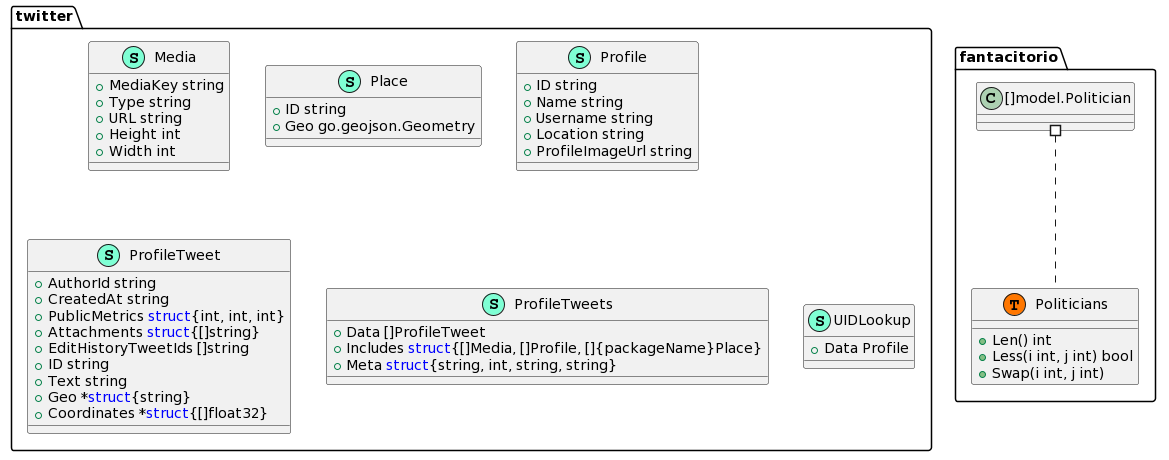
\includegraphics[width=\textwidth]{backend-twitter-fantacitorio}

\section{\emph{Sprint} 0}

\subsection{\emph{Sprint goal}}

Lo sprint goal per lo sprint 0 è la "preparazione" dell'intero progetto.

\subsection{\emph{Sprint backlog}}

Lo sprint backlog è consistito di due storie, entrambe tecniche:



\subsection{\emph{Definition of done}}

\subsection{\emph{Test} di ciascuna storia}

\subsection{\emph{Burndown} dello sprint}

\subsection{Qualità del codice}

\subsection{Retrospettiva con \emph{Essence}}

\section{\emph{Sprint} 1}

\subsection{\emph{Sprint goal}}

\subsection{\emph{Sprint backlog}}

\subsection{\emph{Definition of done}}

\subsection{\emph{Test} di ciascuna storia}

\subsection{\emph{Burndown} dello sprint}

\subsection{Qualità del codice}

\subsection{Retrospettiva con \emph{Essence}}

\section{\emph{Sprint} 2}

\subsection{\emph{Sprint goal}}

\subsection{\emph{Sprint backlog}}

\subsection{\emph{Definition of done}}

\subsection{\emph{Test} di ciascuna storia}

\subsection{\emph{Burndown} dello sprint}

\subsection{Qualità del codice}

\subsection{Retrospettiva con \emph{Essence}}

\section{\emph{Sprint} 3}

\subsection{\emph{Sprint goal}}

\subsection{\emph{Sprint backlog}}

\subsection{\emph{Definition of done}}

\subsection{\emph{Test} di ciascuna storia}

\subsection{\emph{Burndown} dello sprint}

\subsection{Qualità del codice}

\subsection{Retrospettiva con \emph{Essence}}

\section{\emph{Sprint} 4}

\subsection{\emph{Sprint goal}}

\subsection{\emph{Sprint backlog}}

\subsection{\emph{Definition of done}}

\subsection{\emph{Test} di ciascuna storia}

\subsection{\emph{Burndown} dello sprint}

\subsection{Qualità del codice}

\subsection{Retrospettiva con \emph{Essence}}

\section{Processo seguito}

\subsection{Numero e durata degli sprint}

\subsection{Autodescrizione del \emph{team}}

\subsection{Risultato dello Scrumble iniziale}

\subsection{Sintesi dei dati di \emph{Gitinspector}}

\subsection{Retrospettiva finale con \emph{Essence}}

\subsection{Diagramma del \emph{deployment} del prodotto}

\section{Demo}

\section{Artefatti}

\end{document}
